
\subsubsection{模型建立}

针对问题一，本节将从圆柱体几何表示、周期性边界裁剪和电极距离计算三个层面建立导通判定模型。具体过程如下。

\textbf{步骤1：圆柱体的几何表示}

金属A圆柱体由其轴线（两端点连线）和半径定义。轴线方向向量为：
\begin{equation}
\mathbf{v} = \mathbf{p}_2 - \mathbf{p}_1 = (x_2-x_1, y_2-y_1, z_2-z_1)
\end{equation}
圆柱体表面由所有到轴线距离等于$R_A$的点组成。圆柱体表面到空间中任意一点$Q$的最短距离为：
\begin{equation}
d(Q, \text{cyl}) = \max(0, d_{\text{axis}}(Q) - R_A)
\end{equation}
其中，$d_{\text{axis}}(Q)$为点$Q$到轴线的垂直距离，通过点到线段距离公式计算：
\begin{equation}
d_{\text{axis}}(Q) = \|(\mathbf{p}_1 - Q) - t^* \cdot \mathbf{v}\|
\end{equation}
其中$t^* = \text{clip}\left(\frac{(\mathbf{p}_1 - Q) \cdot \mathbf{v}}{\|\mathbf{v}\|^2}, 0, 1\right)$为投影参数。

\textbf{步骤2：周期性边界裁剪}

对圆柱体轴线应用周期性边界条件。在轴线上均匀采样$N_s$个点：
\begin{equation}
\mathbf{s}_k = \mathbf{p}_1 + \frac{k}{N_s}(\mathbf{p}_2 - \mathbf{p}_1), \quad k = 0, 1, \ldots, N_s
\end{equation}
对每个采样点应用周期性映射：
\begin{equation}
\mathbf{s}'_k = ((\mathbf{s}_k + 5000) \bmod 10000) - 5000
\end{equation}
检测相邻采样点间的不连续跳跃（距离$>5000$nm），将轴线分割为若干有效分段。各分段共同构成金属A在微构体内的有效几何表示。

\textbf{步骤3：电极距离计算与导通判定}

对每个有效分段的轴线，计算该分段上各点到电极面的最短距离。到左电极面（$X=-5000$）的表面距离为：
\begin{equation}
d_L = \min_{\mathbf{q} \in \text{seg}} |q_x - (-5000)| - R_A
\end{equation}
同理，到右电极面（$X=+5000$）的表面距离为：
\begin{equation}
d_R = \min_{\mathbf{q} \in \text{seg}} |q_x - 5000| - R_A
\end{equation}

导通判据：若同一圆柱体的各有效分段中，存在某一分段或若干分段的组合使得$d_L \leq d_t$且$d_R \leq d_t$，则该微构体导通。其中$d_t=1.8$nm为隧穿距离。由于圆柱体长度（5000nm）仅为微构体边长（10000nm）的一半，单个圆柱体在绝大多数情况下无法同时触及两侧电极。

综上所述，本节完成了单颗粒导通判定的数学模型建立，接下来将基于此进行求解。

\subsubsection{模型求解}

基于上述模型，本节对附件1中12个金属A颗粒逐一进行导通判定。判定结果如表\ref{tab:问题一结果}所示。

\begin{longtable}{>{\centering\arraybackslash}p{0.06\textwidth}>{\centering\arraybackslash}p{0.16\textwidth}>{\centering\arraybackslash}p{0.16\textwidth}>{\centering\arraybackslash}p{0.16\textwidth}>{\centering\arraybackslash}p{0.12\textwidth}>{\centering\arraybackslash}p{0.10\textwidth}}
  \caption{问题一单颗粒导通判定结果}
  \label{tab:问题一结果} \\
  \toprule
  序号 & 端点1 (nm) & 端点2 (nm) & $d_L$ (nm) & $d_R$ (nm) & 导通 \\
  \midrule
  \endfirsthead
  \caption{问题一单颗粒导通判定结果（续）} \\
  \toprule
  序号 & 端点1 (nm) & 端点2 (nm) & $d_L$ (nm) & $d_R$ (nm) & 导通 \\
  \midrule
  \endhead
  \bottomrule
  \endfoot
  1 & (-5000, -124, -413) & (-2588, 264, -257) & -30.0 & 7558.1 & 否 \\
  2 & (-5000, 261, -46) & (-2698, 420, 142) & -30.0 & 7667.6 & 否 \\
  3 & (-5000, 274, -145) & (-3939, 319, -118) & -30.0 & 8909.2 & 否 \\
  4 & (-4192, 262, -200) & (807, 322, -284) & 777.7 & 4163.4 & 否 \\
  5 & (-2778, -159, -250) & (2215, 98, -281) & 2192.0 & 2754.7 & 否 \\
  6 & (-2262, -250, 442) & (-844, -278, -500) & 2708.0 & 5813.9 & 否 \\
  7 & (-844, -278, -500) & (2733, -346, -353) & 4126.1 & 2237.2 & 否 \\
  8 & (577, -500, -307) & (5000, -472, -258) & 4970.0 & -30.0 & 否 \\
  9 & (1067, 105, -243) & (5000, 274, -145) & 3970.7 & -30.0 & 否 \\
  10 & (2781, 378, -382) & (5000, 66, -280) & 2268.0 & -30.0 & 否 \\
  11 & (2660, -143, 298) & (3661, 34, -112) & 7626.5 & 1309.3 & 否 \\
  12 & (3215, -202, 396) & (5000, -61, -155) & 1785.0 & -30.0 & 否 \\
\end{longtable}

由表\ref{tab:问题一结果}可知，12个配置中导通数为0，导通概率为0\%。其中有6个颗粒的一端位于电极面上（$d_L=-30$nm或$d_R=-30$nm），表明该端表面与电极面接触（距离为负表示圆柱体表面已穿透电极面），但另一端到对侧电极的距离至少为65.7nm（颗粒12），远超1.8nm的隧穿距离。出现的负距离值（$-30$nm）是由于圆柱体底面恰好位于电极面上，圆柱体半径30nm的柱面穿透了电极平面所致。

\begin{figure}[ht]
  \centering
  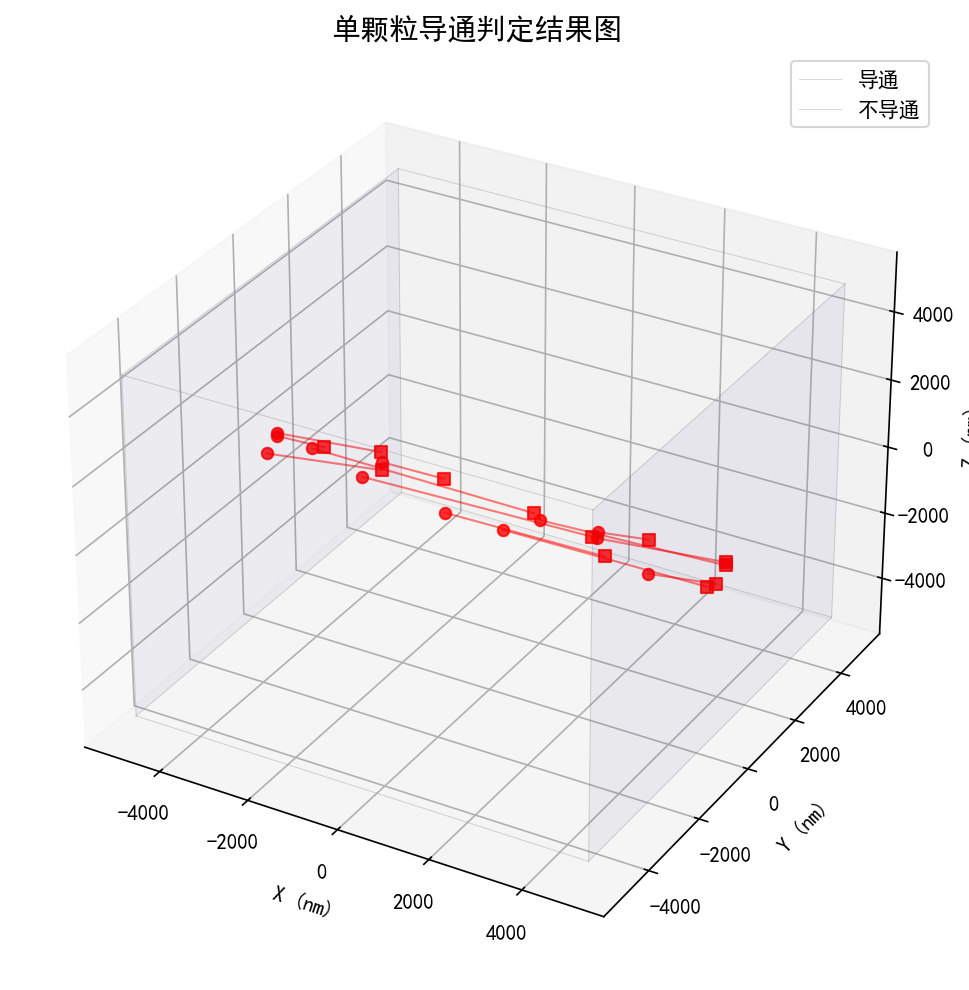
\includegraphics[width=0.8\textwidth]{../求解/问题一/图片/单颗粒导通判定结果图.png}
  \caption{单颗粒导通判定结果3D可视化}
  \label{fig:q1_3d}
\end{figure}

\begin{figure}[ht]
  \centering
  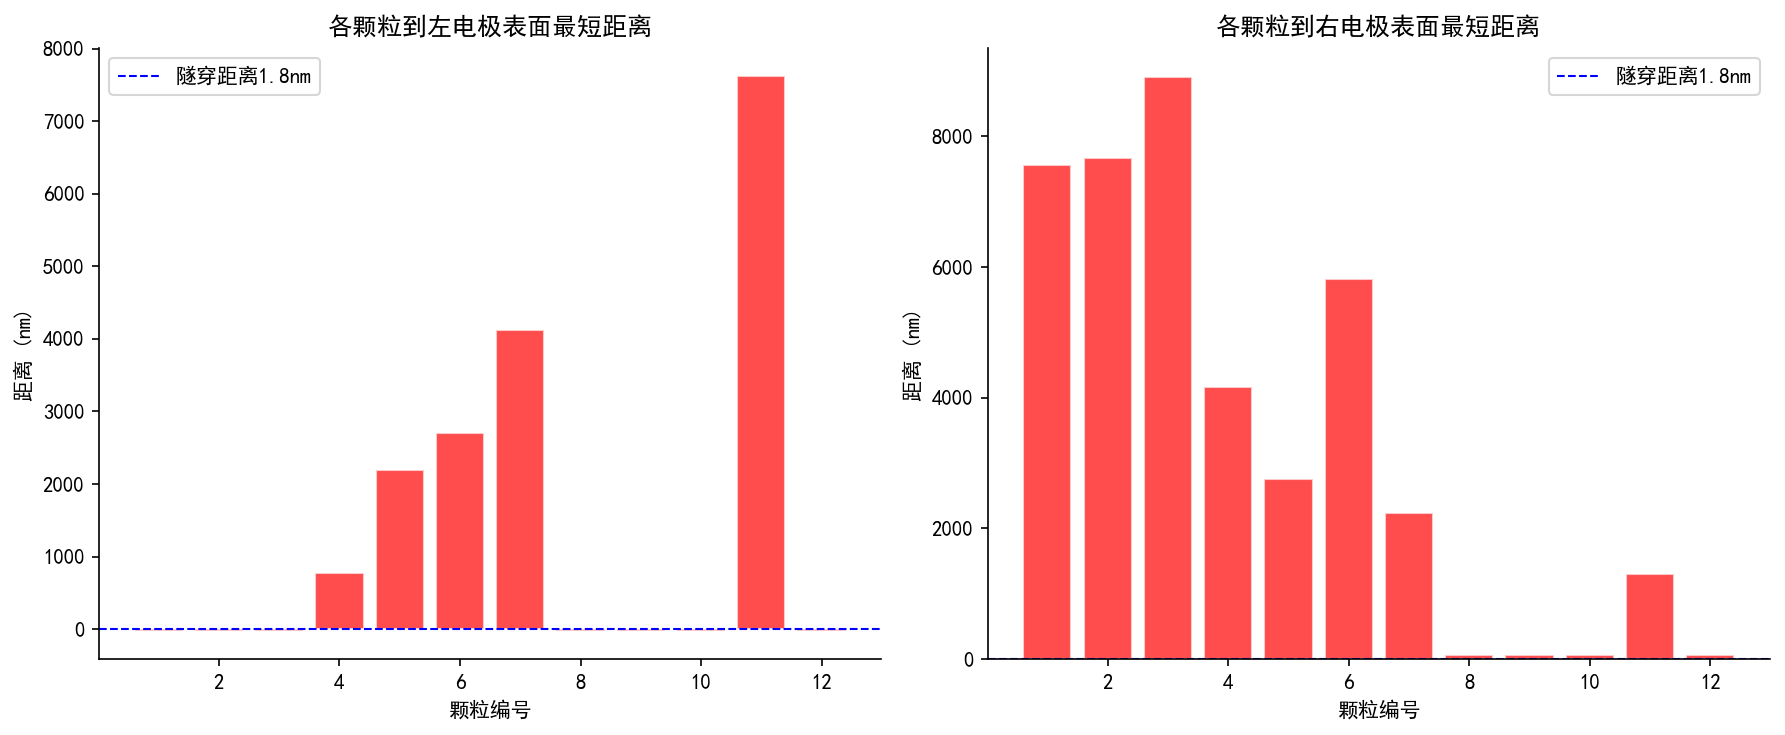
\includegraphics[width=0.8\textwidth]{../求解/问题一/图片/电极距离分布图.png}
  \caption{各颗粒到两侧电极的表面最短距离}
  \label{fig:q1_dist}
\end{figure}

如图\ref{fig:q1_3d}和图\ref{fig:q1_dist}所示，12个颗粒在微构体中分散分布，多数颗粒仅能触及一侧电极或两侧均无法触及。这是由几何约束决定的：金属A圆柱体长度5000nm仅为微构体边长10000nm的一半，单个圆柱体在三维空间中无论如何放置都无法跨越整个微构体宽度。综上所述，问题一判定单个金属A颗粒的导通概率为0\%。
